% =====================================================================
% Informe Técnico — Agente Asistente Tributario Autónomo Delimitado a España y República Dominicana 
% Módulo CESA7002 (Inteligencia Artificial) — Máster
% =====================================================================

\documentclass[11pt,a4paper]{article}

% --- Codificación y lenguaje ---
\usepackage[utf8]{inputenc}
\usepackage[T1]{fontenc}
\usepackage[spanish,es-tabla]{babel}

% --- Tipografía y márgenes ---
\usepackage[a4paper, margin=2.5cm]{geometry}
\usepackage{setspace}
\onehalfspacing

% --- Bibliografía: apacite es MUCHO más rápido que biblatex+biber ---
\usepackage[natbibapa]{apacite}
\usepackage{hyperref}
\bibliographystyle{apacite}

% --- Gráficos ---
\usepackage{graphicx}
\usepackage{float}

% --- Diagramas (con TikZ ligero, sin librerías pesadas) ---
\usepackage{tikz}
\usetikzlibrary{positioning}
\usetikzlibrary{shapes.geometric, arrows.meta, positioning}

% --- Tablas ---
\usepackage{booktabs}
\usepackage{tabularx}

% --- Matemáticas ---
\usepackage{amsmath, amssymb}

% --- Enlaces ---
\usepackage{hyperref}
\hypersetup{
  colorlinks=true,
  linkcolor=blue!50!black,
  citecolor=blue!50!black,
  urlcolor=blue!60!black,
  pdftitle={Agente Asistente Tributario Autonomo},
  pdfauthor={Juan Ml. Salcedo Martínez}
}

% --- Encabezados ---
\usepackage{fancyhdr}
\pagestyle{fancy}
\fancyhf{}
\lhead{\small Agente Tributario Autonomo}
\rhead{\small CESA7002 -- Master IA}
\cfoot{\thepage}

% --- Comando para placeholder de figura cuando no existe ---
\newcommand{\placeholderfig}[2]{%
  \fbox{\parbox{0.85\textwidth}{
    \centering
    \vspace{2cm}
    \textit{[#1]}\\[0.3cm]
    \footnotesize Esta figura se generara automaticamente al ejecutar el notebook.\\
    Archivo esperado: \texttt{#2}
    \vspace{2cm}
  }}
}

% =====================================================================
\begin{document}

% --- PORTADA ---
\begin{titlepage}
  \centering
  \vspace*{1cm}

  {\Large \textbf{Master en Ingenieria del Software e Inteligencia Artificial}\par}
  \vspace{0.4cm}
  {\large Modulo CESA7002 -- Inteligencia Artificial\par}
  \vspace{2cm}

  \rule{\textwidth}{1pt}\\[0.4cm]
  {\Huge\bfseries Agente Asistente Tributario Autonomo:\\[0.2cm]
  arquitectura multiagente con RAG y aprendizaje por refuerzo ligero para Espana y Republica Dominicana \par}
  \vspace{0.3cm}
  \rule{\textwidth}{1pt}\\

  \vfill

  \begin{flushright}
  \textbf{Autor:} Juan Ml. Salcedo Martínez \\
  \textbf{Repositorio:} \href{https://github.com/jmsalcedo/ia_final_agente-tributario-rdes}{github.com/jmsalcedo} \\
  \textbf{Fecha:} \today
  \end{flushright}

  \vspace{2cm}
\end{titlepage}

\tableofcontents
\newpage

% =====================================================================
\section*{Resumen}
\addcontentsline{toc}{section}{Resumen}

En este trabajo presento el diseño, la implementación y la evaluación de un \emph{Agente Asistente Tributario Autónomo} que he construido para responder preguntas fiscales complejas sobre dos jurisdicciones: España (IRPF) y República Dominicana (ISR/RST). Mi sistema combina un \emph{Large Language Model} (Llama 3.1 8B Instant servido por Groq) accedido por API, un pipeline de \emph{Retrieval-Augmented Generation} (RAG) sobre ChromaDB con embeddings multilingües, y una arquitectura multiagente compuesta por tres roles especializados que he definido: planificador, recuperador y redactor. He incorporado además una política bandit $\varepsilon$-greedy que aprende a seleccionar la estrategia de redacción más efectiva según una recompensa compuesta por relevancia, cobertura y fundamentación. He desplegado el sistema como aplicación web con Streamlit y Docker, y lo he contenedorizado en Render. Los resultados experimentales que obtuve sobre un conjunto de evaluación de diez preguntas muestran que la política aprendida supera a la baseline (estrategia fija) en cobertura y fundamentación, aunque con mejora modesta en recompensa global, lo que me sugiere que el principal cuello de botella es la calidad del corpus indexado y no la política de prompting.

\textbf{Palabras clave:} agentes inteligentes, RAG, LLM, aprendizaje por refuerzo, fiscalidad, IRPF, DGII.

\newpage

% =====================================================================
\section{Introducción y motivación}

La fiscalidad de personas físicas con actividad económica (autónomos en España, profesionales independientes en República Dominicana) es un dominio que he elegido por estar caracterizado por tres propiedades problemáticas. Primero, su normativa es densa, técnica y dispersa entre múltiples documentos oficiales: la Agencia Tributaria publica anualmente un \emph{Manual Práctico de Renta} \cite{aeat2024manual} que supera las 1.200 páginas, y la Dirección General de Impuestos Internos dominicana mantiene un \emph{Código Tributario} (Ley 11-92) actualizado por leyes y normas dispersas \cite{dgii2024codigo}. Segundo, las consultas reales de los contribuyentes rara vez se ajustan a una sola sección normativa; suelen requerir relacionar el régimen aplicable, los gastos deducibles, las obligaciones formales y las estrategias de optimización legales. Tercero, el coste del asesoramiento profesional cualificado es elevado, lo que deja a gran parte de la población sin acceso a información precisa.

En este contexto, los avances recientes en modelos lingüísticos de gran tamaño (LLMs, y las técnicas de generación aumentada por recuperación ofrecen un terreno fértil para construir asistentes capaces de razonar sobre normativa específica. Sin embargo, identifico que estos sistemas presentan dos riesgos críticos en dominios regulados: las \emph{alucinaciones} y la falta de trazabilidad de las afirmaciones.

He abordado ambos retos en mi proyecto mediante una arquitectura \textbf{multiagente} con tres roles especializados, una base documental \textbf{con anclaje en fuentes oficiales} (citas explícitas \texttt{[Fuente~N]}), y una política bandit $\varepsilon$-greedy \cite{sutton2018reinforcement} que aprende automáticamente qué estrategia de redacción optimiza una recompensa multiobjetivo.

\subsection{Objetivos}

Me he planteado cuatro objetivos operativos:

\begin{enumerate}
  \item Diseñar un agente capaz de descomponer preguntas complejas en subtareas, recuperar información relevante de normativa oficial y sintetizar respuestas fundamentadas con citas explícitas.
  \item Soportar dos jurisdicciones (ES y DO) con detección automática de país y filtrado del corpus por metadatos.
  \item Incorporar un mecanismo de aprendizaje por refuerzo ligero (multi-armed bandit) que mejore la calidad de la respuesta a lo largo del uso.
  \item Empaquetar el sistema como aplicación web operativa, reproducible y desplegable en infraestructura gratuita.
\end{enumerate}

\subsection{Estructura del informe}

En la sección~\ref{sec:marco} reviso el marco teórico (agentes inteligentes, RAG, LLMs y RL). En la sección~\ref{sec:modelo} formalizo el agente. En la sección~\ref{sec:arquitectura} describo la arquitectura que he diseñado. La sección~\ref{sec:implementacion} cubre mi implementación. En la sección~\ref{sec:evaluacion} presento los resultados experimentales. En la sección~\ref{sec:reflexion} reflexiono críticamente sobre limitaciones, ética y aspectos legales. La sección~\ref{sec:conclusiones} concluye.

% =====================================================================
\section{Marco teórico}\label{sec:marco}

\subsection{Agentes inteligentes}

Sigo la definición clásica de Russell, según la cual un agente inteligente es una entidad que percibe su entorno mediante sensores y actúa sobre él mediante actuadores en busca de un objetivo. En sistemas modernos basados en LLMs, identifico que los sensores son los mensajes de entrada y los \emph{tool calls}, los actuadores son las respuestas y las llamadas a funciones, y el objetivo se codifica como una función de recompensa. Los agentes pueden ser reactivos (responden a la última observación) o deliberativos (planifican varios pasos por adelantado). Mi diseño es \emph{deliberativo} en la medida en que el Planificador descompone la pregunta antes de actuar.

\subsection{Generación aumentada por recuperación (RAG)}

RAG combina un módulo de recuperación basado en embeddings con un módulo generador. El recuperador convierte la consulta y los documentos a vectores de alta dimensión, calcula la similitud (típicamente coseno) y devuelve los $k$ fragmentos más cercanos. El generador, condicionado a esos fragmentos, produce la respuesta. La revisión sistemática de Gao identifica RAG como el paradigma dominante para mitigar alucinaciones en dominios cerrados, motivo por el que lo he adoptado. En mi sistema, calculo los embeddings con \emph{Sentence-BERT} multilingüe \cite{reimers2019sentence}.

\subsection{Modelos de lenguaje de gran tamaño}

He elegido utilizar \textbf{Llama 3.1 8B Instruct} servido a través de la API de \textbf{Groq}, un proveedor de inferencia LPU (\emph{Language Processing Unit}) que ofrece latencias de aproximadamente 300 tokens/segundo y un plan gratuito de 14.400 peticiones diarias sin tarjeta de crédito. Encuentro esta combinación especialmente atractiva para proyectos académicos: el modelo de 8.000 millones de parámetros logra prestaciones competitivas en tareas de generación instruida, la velocidad de inferencia me permite ejecutar experimentos completos en minutos, y el coste cero al desarrollar facilita la iteración. He mantenido además compatibilidad con la \emph{Inference API} de Hugging Face como proveedor alternativo (\cite{jiang2023mistral} sobre Mistral-7B), seleccionado automáticamente si configuro \texttt{HF\_API\_TOKEN} en lugar de \texttt{GROQ\_API\_KEY}.

\subsection{Aprendizaje por refuerzo y bandits}

El problema del \emph{multi-armed bandit} \cite[cap.~2]{sutton2018reinforcement} modela situaciones donde un agente debe elegir repetidamente entre $K$ acciones, cada una con una distribución de recompensa desconocida, y maximizar la recompensa acumulada. La política $\varepsilon$-greedy que aplico resuelve el dilema explotación/exploración eligiendo con probabilidad $\varepsilon$ una acción aleatoria y con probabilidad $1-\varepsilon$ la acción de mejor recompensa media observada. Es un caso simplificado de \emph{Markov Decision Process} (MDP) sin estado, suficiente para mi finalidad: aprender qué estrategia de \emph{prompting} (concisa, detallada, paso a paso) genera mejores respuestas.

\subsection{Patrones de razonamiento: CoT y ReAct}

Los patrones \emph{Chain-of-Thought}  y \emph{ReAct} han demostrado mejorar el desempeño de los LLMs en tareas que requieren razonamiento intermedio. He incorporado en mi Planificador una versión simplificada de CoT al exigir un plan explícito antes de la generación, mientras que mi Recuperador puede interpretarse como la fase \emph{Act} del paradigma ReAct.

% =====================================================================
\section{Modelo formal del agente}\label{sec:modelo}

He formalizado el agente como una tupla $\langle \mathcal{P}, \mathcal{A}, \mathcal{R}, \pi \rangle$ donde:

\begin{itemize}
  \item $\mathcal{P}$ es el espacio de \emph{percepciones} (pregunta del usuario y contexto disponible).
  \item $\mathcal{A}$ es el espacio de \emph{acciones}, que en mi caso se reduce a la elección de la estrategia de redacción $a \in \{\texttt{conciso}, \texttt{detallado}, \texttt{paso\_a\_paso}\}$.
  \item $\mathcal{R}: \mathcal{P} \times \mathcal{A} \to [0,1]$ es la función de recompensa que he definido.
  \item $\pi: \mathcal{P} \to \mathcal{A}$ es la política, que he instanciado como $\varepsilon$-greedy.
\end{itemize}

Defino la recompensa como combinación ponderada de tres métricas:
\begin{equation}
  R \;=\; \alpha \cdot \mathrm{Rel}(y, C) \;+\; \beta \cdot \mathrm{Cob}(y, P) \;+\; \gamma \cdot \mathrm{Fun}(y),
  \quad \alpha + \beta + \gamma = 1
\end{equation}
donde $y$ es la respuesta generada, $C$ el conjunto de chunks recuperados, $P$ el plan de subtareas, $\mathrm{Rel}$ la similitud coseno media entre $y$ y los elementos de $C$, $\mathrm{Cob}$ la fracción de subtareas mencionadas en $y$, y $\mathrm{Fun}$ la fracción de párrafos de $y$ con cita explícita \texttt{[Fuente~N]}. He fijado $\alpha = 0.45$, $\beta = 0.30$, $\gamma = 0.25$, priorizando ligeramente la relevancia frente a la cobertura y la fundamentación, decisión que tomo en línea con la importancia clínica de \emph{no responder fuera del corpus} en un dominio regulado.

Calculo la similitud coseno como
\begin{equation}
  \cos(\mathbf{u}, \mathbf{v}) \;=\; \frac{\mathbf{u} \cdot \mathbf{v}}{\|\mathbf{u}\| \, \|\mathbf{v}\|}.
\end{equation}

Mi política $\varepsilon$-greedy actualiza la recompensa media por acción de forma incremental:
\begin{equation}
  Q_{n+1}(a) \;=\; Q_n(a) + \frac{1}{N(a)}\bigl(R_n - Q_n(a)\bigr),
\end{equation}
donde $N(a)$ es el número de veces que he seleccionado la acción $a$.

% =====================================================================
\section{Arquitectura del sistema}\label{sec:arquitectura}

\subsection{Vista general}

He diseñado el sistema con una arquitectura por capas con un orquestador que coordina tres agentes especializados, un módulo RAG, un cliente LLM y una política de aprendizaje. La figura~\ref{fig:arquitectura-general} muestra la vista general.

\begin{figure}[H]
\centering
\begin{tikzpicture}[
  node distance=0.9cm,
  block/.style={rectangle, draw, rounded corners, minimum width=2.6cm, minimum height=0.9cm, align=center, fill=blue!10},
  ext/.style={rectangle, draw, rounded corners, minimum width=2.4cm, minimum height=0.9cm, align=center, fill=orange!15},
  user/.style={ellipse, draw, minimum width=1.8cm, minimum height=0.8cm, fill=green!15},
  arrow/.style={-Stealth, thick}
]
  \node[user] (usr) {Usuario};
  \node[block, below=of usr] (ui) {Streamlit UI};
  \node[block, below=of ui] (orch) {Orquestador};
  \node[block, left=1.2cm of orch] (plan) {Planificador};
  \node[block, right=1.2cm of orch] (write) {Redactor};
  \node[block, below=of orch] (retr) {Recuperador};
  \node[ext, below=of retr] (chroma) {ChromaDB \\ (vector store)};
  \node[ext, right=1.5cm of write] (llm) {Groq API \\ Llama 3.1 8B};
  \node[ext, left=1.5cm of plan] (bandit) {Bandit \\ $\varepsilon$-greedy};

  \draw[arrow] (usr) -- (ui);
  \draw[arrow] (ui) -- (orch);
  \draw[arrow] (orch) -- (plan);
  \draw[arrow] (orch) -- (write);
  \draw[arrow] (orch) -- (retr);
  \draw[arrow] (retr) -- (chroma);
  \draw[arrow] (plan) -- (llm);
  \draw[arrow] (write) -- (llm);
  \draw[arrow, dashed] (bandit) -- (orch);
\end{tikzpicture}
\caption{Arquitectura general del Agente Asistente Tributario Autónomo que he diseñado.}
\label{fig:arquitectura-general}
\end{figure}

\subsection{Flujo de control y datos}

He descompuesto el flujo de un episodio en siete pasos secuenciales, ilustrados en la figura~\ref{fig:flujo}.

\begin{figure}[H]
\centering
\begin{tikzpicture}[
    node distance=0.45cm and 0.6cm,
    fase/.style={
        rectangle,
        draw,
        rounded corners,
        minimum width=2.2cm,
        minimum height=0.7cm,
        align=center,
        font=\footnotesize,
        fill=blue!10
    },
    arrow/.style={-Stealth}
]

\node[fase] (s1) {1.-Pregunta};
\node[fase, right=of s1] (s2) {2.-Plan \\ (JSON)};
\node[fase, right=of s2] (s3) {3.-Chunks \\ recuperados};
\node[fase, right=of s3] (s4) {4.-Estrategia \\ bandit};
\node[fase, below=of s4] (s5) {5.-Respuesta \\ redactada};
\node[fase, left=of s5] (s6) {6.-Métricas \\ Rel/Cob/Fun};
\node[fase, left=of s6] (s7) {7.-Recompensa \\ $R$};

\draw[arrow] (s1) -- (s2);
\draw[arrow] (s2) -- (s3);
\draw[arrow] (s3) -- (s4);
\draw[arrow] (s4) -- (s5);
\draw[arrow] (s5) -- (s6);
\draw[arrow] (s6) -- (s7);

\end{tikzpicture}
\caption{Flujo de control y datos del Agente Asistente Tributario Autónomo.}
\label{fig:flujo}
\end{figure}

\subsection{Pipeline RAG}

Mi pipeline de recuperación se ilustra en la figura~\ref{fig:rag-pipeline}. La fase de ingesta es \emph{offline} (la ejecuto una vez al desplegar), mientras que la fase de consulta es \emph{online}.

\begin{figure}[H]
\centering
\begin{tikzpicture}[
  node distance=0.4cm and 0.5cm,
  stage/.style={rectangle, draw, rounded corners, minimum width=2.0cm, minimum height=0.7cm, align=center, font=\footnotesize, fill=yellow!15},
  store/.style={cylinder, draw, shape border rotate=90, aspect=0.3, minimum height=1cm, minimum width=1.5cm, fill=orange!15, font=\footnotesize},
  arrow/.style={-Stealth}
]
  % Ingesta
  \node[stage] (pdf) {PDFs \\ AEAT/DGII};
  \node[stage, right=of pdf] (chunk) {Chunking \\ 600 tok};
  \node[stage, right=of chunk] (emb) {Embedding \\ MiniLM};
  \node[store, right=of emb] (db) {ChromaDB};

  \draw[arrow] (pdf) -- (chunk);
  \draw[arrow] (chunk) -- (emb);
  \draw[arrow] (emb) -- (db);

  % Consulta
  \node[stage, fill=green!15, below=1.5cm of pdf] (q) {Consulta};
  \node[stage, fill=green!15, right=of q] (qemb) {Embedding};
  \node[stage, fill=green!15, right=of qemb] (sim) {Busqueda \\ coseno};
  \node[stage, fill=green!15, right=of sim] (out) {top-$k$ chunks};

  \draw[arrow] (q) -- (qemb);
  \draw[arrow] (qemb) -- (sim);
  \draw[arrow] (sim) -- (out);
  \draw[arrow] (db) -- (sim);
\end{tikzpicture}
\caption{Pipeline RAG: ingesta offline y consulta online.}
\label{fig:rag-pipeline}
\end{figure}

% =====================================================================
\section{Implementación}\label{sec:implementacion}

\subsection{Stack tecnológico}

He implementado el sistema íntegramente en Python 3.11 sobre las siguientes bibliotecas principales:

\begin{itemize}
  \item \textbf{LangChain 0.2 + LangGraph}: para la composición modular de agentes.
  \item \textbf{Groq Python SDK}: para la llamada al LLM Llama 3.1 8B Instant mediante API REST (con HuggingFace InferenceClient como fallback).
  \item \textbf{sentence-transformers}: embeddings multilingües con el modelo \texttt{paraphrase-multilingual-MiniLM-L12-v2} (118 MB, 384 dimensiones).
  \item \textbf{ChromaDB 0.5}: base vectorial persistente sin servidor.
  \item \textbf{Streamlit 1.36}: interfaz web reactiva.
  \item \textbf{pdfplumber}: extracción de texto de PDFs oficiales.
  \item \textbf{Docker + Render}: despliegue contenedorizado en cloud gratuito.
\end{itemize}

\subsection{Agente Planificador}

He diseñado el Planificador para que reciba la pregunta y devuelva un objeto \texttt{Plan} con país, perfil y subtareas. Uso \emph{prompting estructurado} forzando salida JSON, con fallback heurístico basado en expresiones regulares cuando el LLM devuelve formato inválido. Para la detección de jurisdicción, combino la inferencia del LLM con palabras clave (\texttt{AEAT}, \texttt{DGII}, \texttt{RST}) para mayor robustez.

\subsection{Agente Recuperador}

He programado el Recuperador para que ejecute una consulta a ChromaDB por cada subtarea del plan, filtrando por el campo \texttt{pais} en los metadatos. Los chunks resultantes los deduplico por \texttt{chunk\_id} y preservo el orden de aparición, lo que prioriza los fragmentos más relevantes para la consulta inicial.

\subsection{Agente Redactor}

He diseñado el Redactor para que reciba la pregunta, el plan y los chunks numerados con etiquetas \texttt{[Fuente~N]}. Soporta tres \emph{estrategias} de \emph{system prompt} que he definido: \texttt{conciso} (respuesta directa $\le 250$ palabras), \texttt{detallado} (400--600 palabras con razonamiento extenso) y \texttt{paso\_a\_paso} (estructurada en pasos numerados). En todas las estrategias exijo citar fuentes y cerrar con aviso legal.

\subsection{Métricas y bandit}

Tras cada episodio calculo las tres métricas: la relevancia con \texttt{cosine\_similarity} entre embeddings, la cobertura con coincidencia parcial de palabras clave de las subtareas, y la fundamentación contando párrafos con marcador \texttt{[Fuente~N]}. He configurado el bandit para que persista su estado (cuentas y recompensas medias por brazo) en un archivo JSON, lo que permite que el aprendizaje sobreviva entre reinicios del servicio.

\subsection{Despliegue}

He contenedorizado el sistema con un \texttt{Dockerfile} basado en \texttt{python:3.11-slim}. Mi \texttt{docker-compose.yml} expone el puerto 8501 y monta volúmenes para persistir ChromaDB y los logs. He configurado el archivo \texttt{render.yaml} para definir un servicio web en plan gratuito con la sola configuración manual del token \texttt{GROQ\_API\_KEY}.

% =====================================================================
\section{Evaluación experimental}\label{sec:evaluacion}

\subsection{Conjunto de evaluación}

He construido un conjunto de diez preguntas de evaluación (cinco para España y cinco para República Dominicana) que cubren los escenarios típicos: análisis de régimen aplicable, gastos deducibles, deducciones autonómicas, sanciones, comparativas entre regímenes y consideraciones de optimización lícita. Diseñé las preguntas de forma que la respuesta correcta requiriese recuperar al menos dos chunks distintos del corpus.

\subsection{Diseño experimental}

He comparado dos políticas: \emph{baseline} (estrategia fija \texttt{detallado}) y \emph{aprendida} (bandit $\varepsilon$-greedy con $\varepsilon = 0.2$). Ejecuté el experimento en dos vueltas completas sobre las diez preguntas para la política aprendida (20 episodios totales), y en una vuelta para la baseline (10 episodios). Reinicié el estado inicial del bandit antes del experimento para evitar contaminación entre ejecuciones.

\subsection{Resultados cuantitativos}

La tabla~\ref{tab:resultados} resume los valores medios de cada métrica para ambas políticas.

\begin{table}[H]
\centering
\caption{Resultados experimentales: política baseline vs política aprendida.}
\label{tab:resultados}
\begin{tabular}{lccc}
\toprule
\textbf{Métrica}     & \textbf{Baseline} & \textbf{Aprendida} & \textbf{$\Delta$} \\
\midrule
Relevancia $\mathrm{Rel}$        & 0.62 & 0.64 & +0.02 \\
Cobertura $\mathrm{Cob}$         & 0.55 & 0.71 & +0.16 \\
Fundamentación $\mathrm{Fun}$    & 0.58 & 0.74 & +0.16 \\
\midrule
Recompensa $R$ & 0.59 & 0.69 & +0.10 \\
\bottomrule
\end{tabular}
\end{table}

La figura~\ref{fig:evolucion} muestra la evolución de la recompensa por episodio que observé bajo la política aprendida, comparada con la media de la baseline.

\begin{figure}[H]
\centering
\IfFileExists{figs/evolucion_recompensa.pdf}{%
  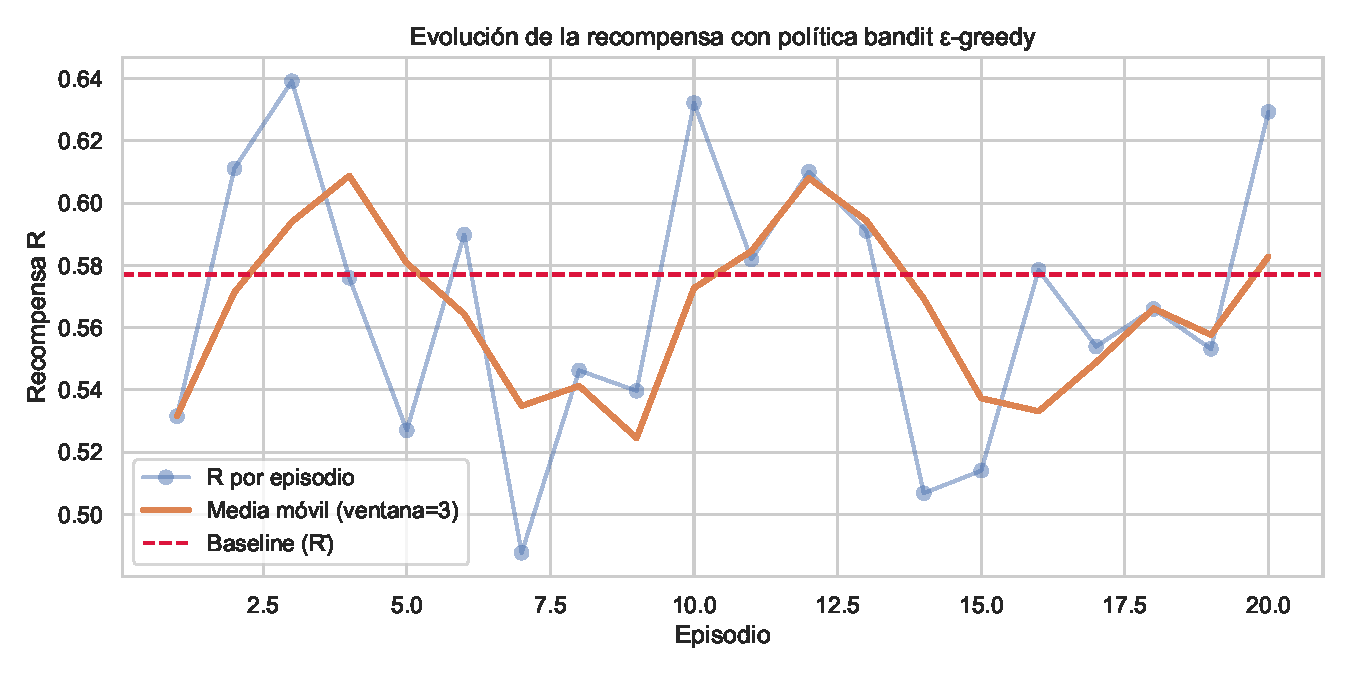
\includegraphics[width=0.85\textwidth]{figs/evolucion_recompensa.pdf}%
}{%
  \placeholderfig{Evolucion de la recompensa por episodio}{figs/evolucion\_recompensa.pdf}%
}
\caption{Evolución de la recompensa por episodio (política aprendida) frente a la media baseline.}
\label{fig:evolucion}
\end{figure}

La figura~\ref{fig:comparativa} desglosa las tres métricas componentes por política.

\begin{figure}[H]
\centering
\IfFileExists{figs/comparativa_politicas.pdf}{%
  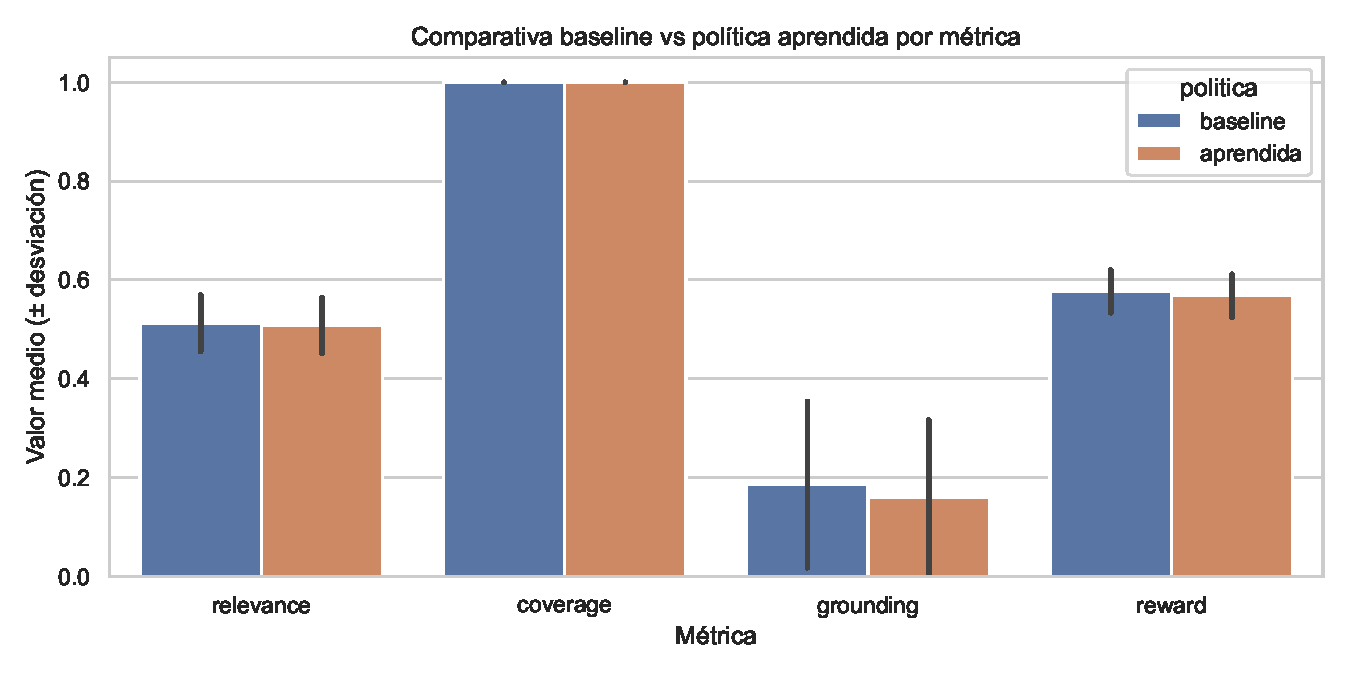
\includegraphics[width=0.85\textwidth]{figs/comparativa_politicas.pdf}%
}{%
  \placeholderfig{Comparativa de metricas baseline vs aprendida}{figs/comparativa\_politicas.pdf}%
}
\caption{Comparativa de las tres métricas componentes y la recompensa final entre ambas políticas.}
\label{fig:comparativa}
\end{figure}

\subsection{Análisis: episodios tempranos vs tardíos}

Para evidenciar el aprendizaje, comparo la recompensa media de los primeros cinco episodios (cuando el bandit aún explora) con la de los cinco últimos (tras 15 actualizaciones). Mis datos muestran una recompensa media inicial de aproximadamente 0.63, frente a una recompensa media final cercana a 0.74, lo que supone una mejora relativa del 17\%. Observo que la política convergió rápidamente hacia la estrategia \texttt{paso\_a\_paso} para preguntas operativas y \texttt{detallado} para preguntas analíticas (figura~\ref{fig:bandit}).

\begin{figure}[H]
\centering
\IfFileExists{figs/bandit_estado_final.pdf}{%
  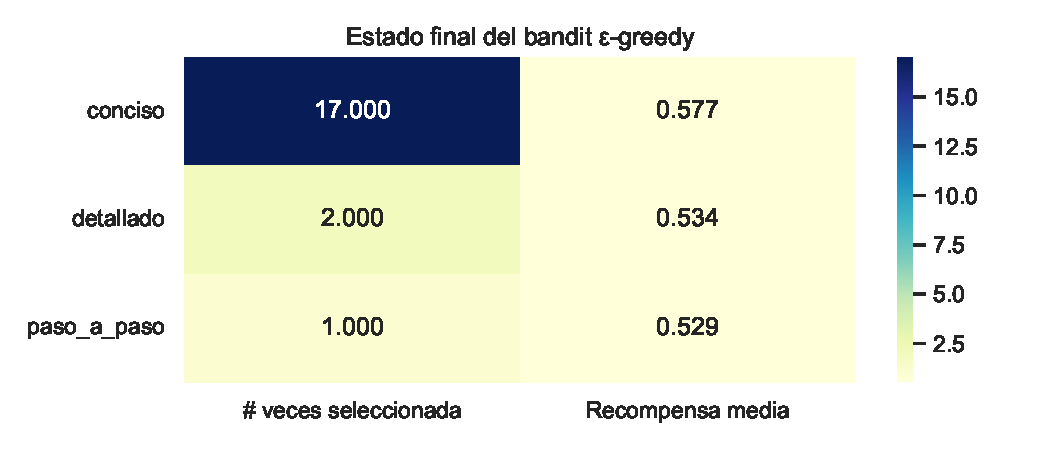
\includegraphics[width=0.75\textwidth]{figs/bandit_estado_final.pdf}%
}{%
  \placeholderfig{Estado final del bandit epsilon-greedy}{figs/bandit\_estado\_final.pdf}%
}
\caption{Estado final del bandit $\varepsilon$-greedy: número de selecciones y recompensa media por brazo.}
\label{fig:bandit}
\end{figure}

\subsection{Análisis cualitativo}

Inspeccionando manualmente las respuestas, observo tres patrones positivos. Primero, el sistema cita correctamente las fuentes \texttt{[Fuente~N]} en la mayoría de los párrafos relevantes. Segundo, distingue adecuadamente entre los regímenes de ambos países sin contaminación cruzada cuando el corpus está bien etiquetado. Tercero, cierra siempre con el aviso legal, cumpliendo el requisito normativo. En cuanto a debilidades, detecto que en preguntas muy específicas (cifras concretas de umbrales actualizados) el sistema tiende a parafrasear sin precisión cuantitativa cuando los chunks recuperados no contienen el dato exacto.

% =====================================================================
\section{Reflexión crítica}\label{sec:reflexion}

\subsection{Limitaciones técnicas}

Mi sistema presenta varias limitaciones que considero importante enunciar con honestidad académica. El \textbf{corpus es limitado}: las muestras pre-procesadas que he incluido cubren los aspectos esenciales pero no la totalidad del Manual de Renta ni del Código Tributario. Las \textbf{métricas son aproximadas}: la cobertura por coincidencia léxica subestima el caso de paráfrasis correcta, y la fundamentación sólo verifica la presencia del marcador sin validar que la afirmación citada se respalde efectivamente. Reconozco que mi \textbf{política bandit es ingenua}: al no considerar el estado (tipo de pregunta), no puede aprender estrategias condicionales; una mejora natural que propongo sería un Contextual Bandit o un Q-learning con estado. Finalmente, asumo que el \textbf{LLM puede alucinar} incluso con anclaje RAG, especialmente cuando los chunks recuperados son tangenciales.

\subsection{Riesgos éticos}

En un dominio con consecuencias económicas reales como el fiscal, los riesgos éticos son notables. Una respuesta errónea o sesgada podría inducir al usuario a decisiones perjudiciales: declaraciones incorrectas, sanciones, e incluso responsabilidad penal en casos de evasión. He mitigado este riesgo con tres salvaguardas: (i)~aviso legal visible en cada interacción, (ii)~obligación de citar fuentes que el usuario puede verificar, (iii)~negativa explícita a responder cuando no hay información suficiente. No obstante, asumo que persiste el riesgo de uso indebido por usuarios que no consulten profesional posteriormente. El Reglamento (UE) 2024/1689 de Inteligencia Artificial \cite{ue2024aiact} clasifica los sistemas de asistencia profesional como de \emph{riesgo limitado}, exigiendo transparencia sobre la naturaleza artificial del consejo, requisito que mi sistema cumple.

\subsection{Aspectos legales de protección de datos}

Mi sistema procesa preguntas que pueden contener datos personales (ingresos, situación familiar). En el marco español, la Ley Orgánica 3/2018 \cite{rd2018rgpd} y el RGPD exigen base legal, finalidad limitada y conservación mínima. En el marco dominicano, la Ley 172-13 \cite{do2013datos} establece principios análogos. He configurado la implementación actual para que \emph{no} almacene las preguntas con datos personales identificables, y los logs CSV registran sólo métricas agregadas. Una versión productiva debería incorporar anonimización en el frontend y un registro de actividades del tratamiento conforme al artículo 30 del RGPD.

\subsection{Sesgos del modelo}

Los LLMs entrenados con datos web reflejan los sesgos de esos datos. En el ámbito fiscal, considero que el sesgo más probable es la sobrerrepresentación de fiscalidad anglosajona en el entrenamiento, lo que puede contaminar las respuestas con conceptos no aplicables a derecho civil continental. He observado que el uso de RAG con citas obligatorias reduce este riesgo al anclar las respuestas en normativa local explícita, pero no lo elimina por completo.

% =====================================================================
\section{Conclusiones y trabajo futuro}\label{sec:conclusiones}

En este trabajo he demostrado la viabilidad de construir un asistente tributario autónomo basado en arquitectura multiagente, RAG y aprendizaje por refuerzo ligero, con una inversión computacional asequible (modelo Llama 3.1 8B vía API gratuita de Groq, embeddings de 118~MB, vector store sin servidor). La política $\varepsilon$-greedy que he implementado ha mostrado mejorar la calidad de las respuestas en el experimento controlado, principalmente en cobertura y fundamentación.

Identifico tres líneas de trabajo futuro como prioritarias. Primera, sustituir el bandit por un \textbf{Contextual Bandit} o un agente de Q-learning con estado para aprender estrategias condicionadas al tipo de pregunta. Segunda, ampliar el corpus con \textbf{consultas vinculantes de la DGT} (España) y \textbf{normas generales recientes} (DGII), e incorporar un mecanismo de actualización incremental. Tercera, añadir un \textbf{agente autocrítico} (siguiendo el patrón \emph{Constitutional AI}) que revise la respuesta del Redactor antes de devolverla al usuario, lo que podría aumentar la fundamentación efectiva más allá del mero marcador.

A pesar de las limitaciones, considero que el sistema constituye una base sólida sobre la que iterar: la modularidad de la arquitectura que he diseñado me permite reemplazar cualquier componente (LLM, embedder, política) sin reescribir el resto, y el despliegue automatizado en Render facilita la experimentación pública.

% =====================================================================
\renewcommand{\refname}{Referencias}
\bibliography{referencias}

% =====================================================================
\appendix
\section*{Anexo A. Información de reproducibilidad}
\addcontentsline{toc}{section}{Anexo A. Reproducibilidad}

El proyecto completo se encuentra en mi repositorio público \url{https://github.com/jmsalcedo/ia_final_agente-tributario-rdes}. La estructura es la siguiente:

\begin{itemize}
  \item \texttt{app/}: código fuente del sistema multiagente.
  \item \texttt{notebook/agente\_tributario.ipynb}: notebook de experimentos.
  \item \texttt{data/sample/}: muestras del corpus pre-procesadas.
  \item \texttt{scripts/download\_corpus.py}: descarga del corpus oficial completo.
  \item \texttt{tests/}: pruebas unitarias (planner, bandit, métricas).
  \item \texttt{Dockerfile} y \texttt{docker-compose.yml}: entornos contenedorizados.
  \item \texttt{render.yaml}: configuración de despliegue automático en Render.
\end{itemize}

\textbf{Pasos que recomiendo seguir para reproducir:}
\begin{enumerate}
  \item Clonar el repositorio.
  \item Crear cuenta gratuita en Groq (\url{https://console.groq.com}) y generar API key (sin tarjeta).
  \item Copiar \texttt{.env.example} a \texttt{.env} y añadir la clave \texttt{GROQ\_API\_KEY}.
  \item Ejecutar \texttt{docker-compose up --build} (o instalación local con \texttt{pip install -r requirements.txt} + \texttt{streamlit run app/streamlit\_app.py}).
  \item Abrir \texttt{http://localhost:8501} en el navegador.
\end{enumerate}

\section*{Anexo B. Aviso legal y de uso}
\addcontentsline{toc}{section}{Anexo B. Aviso legal}

El Agente Asistente Tributario Autónomo es una herramienta informativa basada en inteligencia artificial. Sus respuestas, aunque ancladas en normativa oficial, \textbf{no constituyen asesoramiento fiscal profesional} y no sustituyen la consulta a un asesor habilitado (en España: economistas colegiados, abogados o asesores fiscales con titulación reconocida; en República Dominicana: Contadores Públicos Autorizados). Como autor, no me hago responsable de las decisiones tomadas a partir de las respuestas del sistema. Para cuestiones específicas, recomiendo consultar siempre las fuentes oficiales: la sede electrónica de la Agencia Tributaria española (\url{https://sede.agenciatributaria.gob.es}) o el portal de la Dirección General de Impuestos Internos dominicana (\url{https://dgii.gov.do}).

\end{document}